
\begin{figure}[H]
  \centering
  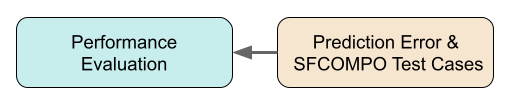
\includegraphics[width=0.7\linewidth]{./chapters/exp1/methodology4.png}
  \caption{Fourth portion of the flowchart from Figure \ref{fig:method} being 
           described in this section.}
\end{figure}

\subsection{Random Error Impacts on Prediction}
\label{sec:randerr}
As previously introduced in Section \ref{sec:testerr}, the prediction
performance is measured by evaluating the accuracy of the reactor type
classification or the error of the regression cases (burnup, \gls{U235}
enrichment, cooling time).  These performance metrics for all four prediction
types are compared across the three algorithms used: \textit{k}-nearest
neighbors (denoted in plots as \textit{kNN}), decision trees (denoted in plots
as \textit{Dec Tree} or \textit{DTree}), and \gls{MLL} calculations.  To judge
the degradation of predictions of the algorithms with increasing nuclide mass
measurement error (i.e., reduced information quality, detailed in section
\ref{sec:inforeduc1}), four plots are made with the introduced error on the
\textit{x}-axis and a prediction performance metric on the \textit{y}-axis.
Shown in Figure \ref{fig:randerr}, the \textit{y}-axis is always oriented so
that lower is poorer performance and higher is better performance. This is why
Figures \ref{fig:randerrB}--\ref{fig:randerrD} present a negative error on the
\textit{y}-axis.
\todo[inline]{In order to have consistency in plot presentation w future plots,
the plots in this section have a small delta-x to show error bars that are
otherwise hard to see.  Since the x-axis is continuous, this may force a return
to using the fill-between to visualize error bands instead.}

Figure \ref{fig:randerrA} shows the balanced accuracy of reactor type
classification, where a score of $1$ is perfect prediction and a score of $0$
is random classification. The error bars reflect a 99\% confidence interval.
While the two scikit-learn algorithms follow a very similar path of decreased
accuracy as the error increases, the \gls{MLL} calculation approach appears to
be more robust to the nuclide mass measurement error. This behavior is seen in
all four plots in Figure \ref{fig:randerr}. Another interesting result is that
the \gls{MLL} calculation performs slightly worse for low errors. If the
expected measurement errors of nuclide masses in a training database or in a
test sample can be guaranteed to be better than ~2\%, the \gls{MLL} calculation
is no longer the obvious preferred choice for reactor type prediction.

Although the balanced accuracy score provides slightly better information about
classification performance for an imbalanced data set (the training set is
26.8\% \gls{PWR}, 71.6\% \gls{BWR}, and 1.5\% \gls{PHWR}), it still does not
provide much detail about what is being misclassified. To probe this further,
Figure \ref{fig:cm_nuc29} shows two sets of confusion matrices.  The diagonal
squares are the fraction of true positives for each reactor type, where the
predicted label (\textit{x}-axis) is equal to the true label (\textit{y}-axis).
The off diagonal squares are the fraction of false positives for each reactor
type, where the predicted label is something other than the true label. In
addition to the numbers being included in the matrices, a colorbar provides
perceptially uniform shading for these true positive and false positive
fractions. 

In Figure \ref{fig:cm_nuc29_01}, the three algorithms are presented for the 1\%
random error case. In Figure \ref{fig:randerrA}, one can see these three data
points on the plot clustered near the top showing almost-perfect performance.
(A reminder that the true positive fractions in the confusion matrices do not
map directly to the balanced accuracy score, which puts more weight on the
underrepresented classes.) The confusion matrices give more dimension to this
near-perfect reactor type classification performance. The majority of the
misclassification is in \gls{PWR}s being classified as \gls{BWR}s: 0.4\% for
\textit{k}-nearest neighbors and decision trees, and 1.6\% for \gls{MLL}
calculations. Although, there are also some \gls{BWR}s that are misclassified
as \gls{PWR}s: 0.1\% for \textit{k}-nearest neighbors and decision trees, and
0.5\% for \gls{MLL} calculations. The \gls{PWR}/\gls{BWR} distinction is known
to be a difficult problem\todo{find citation}, so the correct \gls{PHWR}
classifications are not particularly notable for this discussion.

Figure \ref{fig:cm_nuc29_10} shows confusion matrices for the three algorithms
for the 10\% random error case. In Figure \ref{fig:randerrA}, one can see these
three data points on the plot, where the \gls{MLL} point is near a balanced
accuracy score of 1, and the scikit-learn algorithms both have score of around
0.93. As with the 1\% error case, the majority of the misclassification is in
\gls{PWR}s being classified as \gls{BWR}s: 11.0\% for \textit{k}-nearest
neighbors, 10.3\% for decision trees, and 1.7\% for \gls{MLL} calculations.
The \gls{BWR}s are being misclassified as \gls{PWR}s at the following
percentages: 3.4\% for \textit{k}-nearest neighbors, 3.7\% for decision trees,
and 0.5\% for \gls{MLL} calculations. Note how the performance of the \gls{MLL}
calculations are nearly the same for both error levels, which is shown by the 
\gls{MLL} line in Figure \ref{fig:randerrA}.

Figure \ref{fig:randerrB} demonstrates the burnup prediction performance.  As
mentioned, the \textit{x}-axis is negative \gls{MAPE} so that higher is always
better.  The error bars reflect one standard deviation of the average
percentage errors.  Again, the \gls{MLL} method is robust to training set error
but performs slightly worse at low error values.  All three methods calculate
burnup with a maximum error of 5\% at 20\% error in the training set.  While it
is difficult to draw a baseline, this minimum performance level can serve as a
benchmark for the work presented in Chapter \ref{ch:exp2}. 

\begin{figure}[!hbt]
    \centering
    \begin{subfigure}[b]{0.49\textwidth}
        \centering
        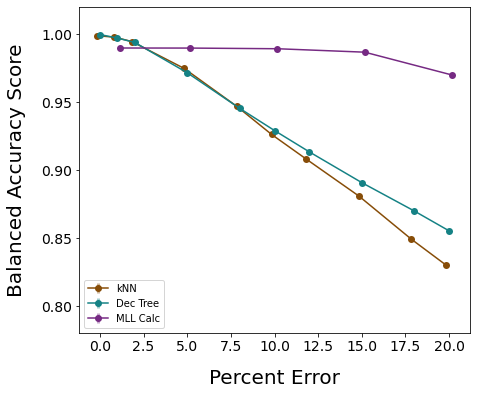
\includegraphics[width=\textwidth]{./chapters/exp1/randerr_compare_nuc29_BalAcc_rxtr.png}
        \caption{Balanced accuracy of reactor type classification with respect 
                 to random error.}
        \label{fig:randerrA}
    \end{subfigure}
    \hfill
    \begin{subfigure}[b]{0.49\textwidth}
        \centering
        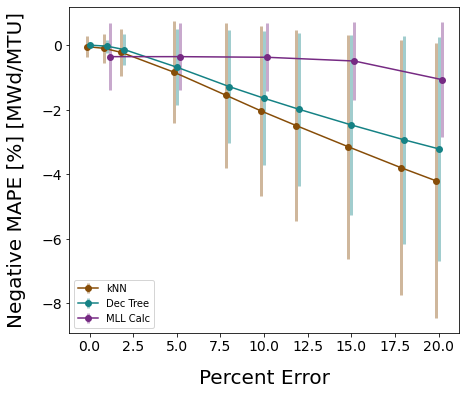
\includegraphics[width=\textwidth]{./chapters/exp1/randerr_compare_nuc29_MAPE_burn.png}
        \caption{Negative \gls{MAPE} of burnup regression with respect to 
                 random error.}
        \label{fig:randerrB}
    \end{subfigure}
    \vskip\baselineskip
    \begin{subfigure}[b]{0.49\textwidth}
        \centering
        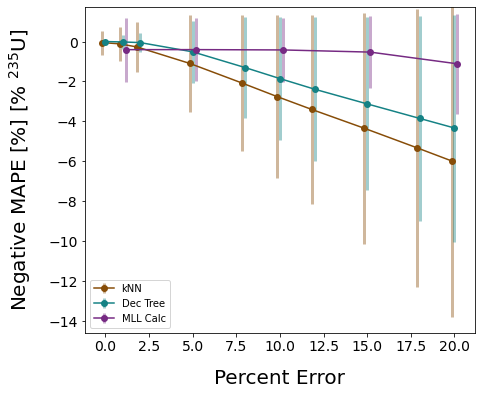
\includegraphics[width=\textwidth]{./chapters/exp1/randerr_compare_nuc29_MAPE_enri.png}
        \caption{Negative \gls{MAPE} of \gls{U235} enrichment regression with 
                 respect to random error.}
        \label{fig:randerrC}
    \end{subfigure}
    \hfill
    \begin{subfigure}[b]{0.49\textwidth}
        \centering
        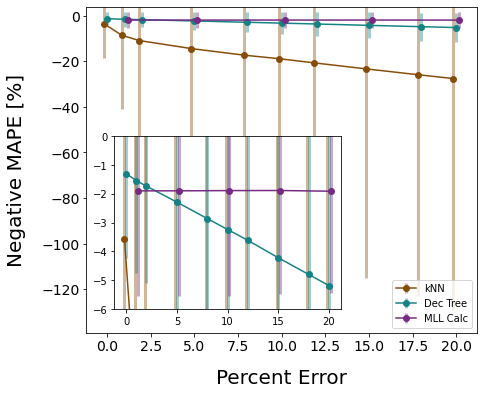
\includegraphics[width=\textwidth]{./chapters/exp1/randerr_compare_nuc29_MAPE_cool.png}
        \caption{Negative \gls{MAPE} of time since irradiation regression with 
                 respect to random error.} 
        \label{fig:randerrD}
    \end{subfigure}
    \caption{Prediction performance of reactor type, burnup, enrichment, and 
             time since irradiation with respect to decreasing information
             quality in the form of uniform/random error applied to the nuclide 
             mass measurements in the training set.}
    \label{fig:randerr}
\end{figure}

\begin{figure}[!htb]
    \centering
    \begin{subfigure}[b]{\textwidth}
        \centering
        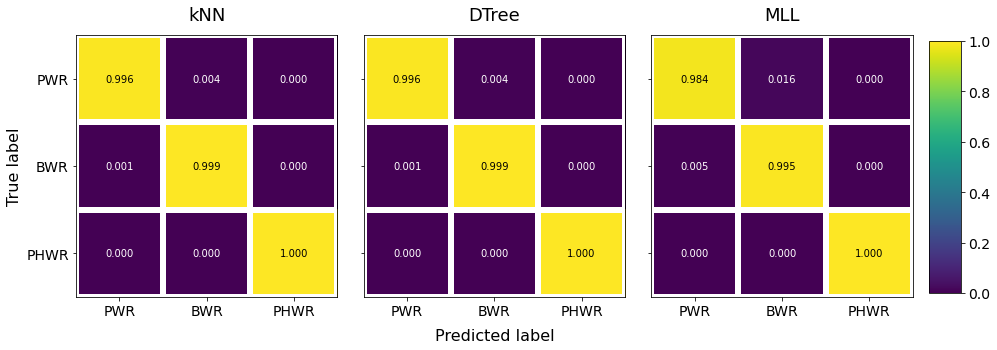
\includegraphics[width=\textwidth]{./chapters/exp1/confusion_matrix_nuc29_err01.png}
        \caption{Confusion matrices for 1\% error for each algorithm.}
        \label{fig:cm_nuc29_01}
    \end{subfigure}
    \vskip\baselineskip
    \begin{subfigure}[b]{\textwidth}
        \centering
        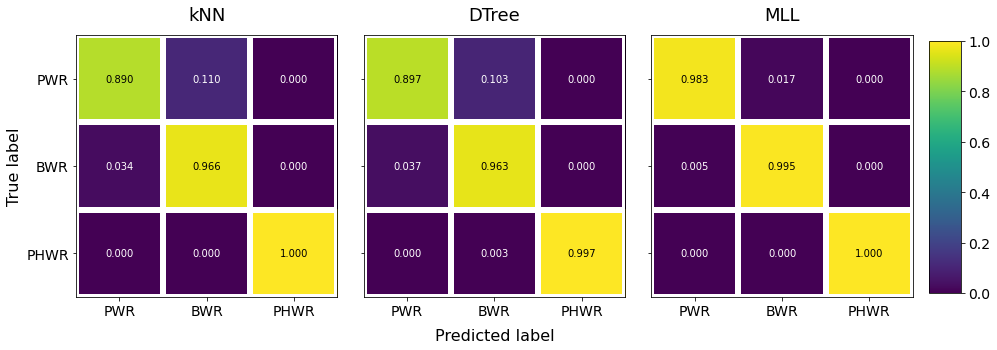
\includegraphics[width=\textwidth]{./chapters/exp1/confusion_matrix_nuc29_err10.png}
        \caption{Confusion matrices for 10\% error for each algorithm.}
        \label{fig:cm_nuc29_10}
    \end{subfigure}
    \caption{Confusion matrices for reactor type prediction for each algorithm 
             at two training set error levels: 1\% and 10\%.}
    \label{fig:cm_nuc29}
\end{figure}

Figure \ref{fig:randerrC} shows the trend of \gls{U235} enrichment prediction
with increasing error in the nuclide mass training set.  The error bars reflect
one standard deviation of the average percentage errors, and the behavior of
the \gls{MLL} method in Figure \ref{fig:randerrB} versus the scikit-learn
algorithms is the same here.  The maximum \gls{MAPE} is about 6\% at 20\%
training set error. 

Last, the time since irradiation prediction performance for the three
algorithms with respect to increasing nuclide mass error is pictured in Figure
\ref{fig:randerrD}.  The error bars reflect one standard deviation of the
average percentage errors.  The behavior of \textit{k}-nearest neighbors is
unique here versus the previous two regression categories; whereas the maximum
prediction \gls{MAPE}s remain under about 6\% for both the decision tree and
\gls{MLL} methods, the maximum error of \textit{k}-nearest neighbors reaches
nearly 30\% at 20\% nuclide mass error. \todo[inline]{1. do I need more ticks
on these y-axes?  2. I'm not sure why this is the case, and have not found a
way to figure this out yet. In previous iterations of the experiment, all
methods performed worse on the cooling time.  But now that is not the case and
it's only kNN performing significantly worse} 

\noindent \textbf{Model Generalization}

\begin{figure}[!htb]
    \centering
    \begin{subfigure}[b]{0.49\textwidth}
        \centering
        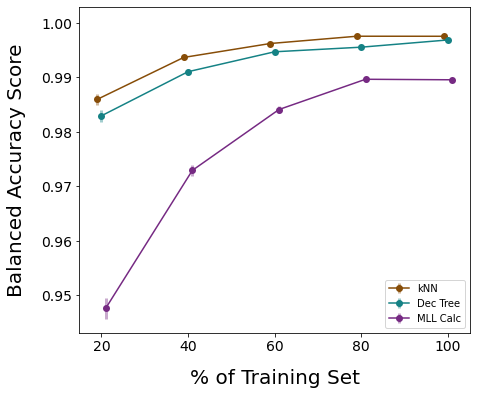
\includegraphics[width=\textwidth]{./chapters/exp1/learncurve_nuc29_BalAcc_rxtr.png}
        \caption{Balanced accuracy of reactor type classification with respect 
                 to training set size.}
        \label{fig:learnsA}
    \end{subfigure}
    \hfill
    \begin{subfigure}[b]{0.49\textwidth}
        \centering
        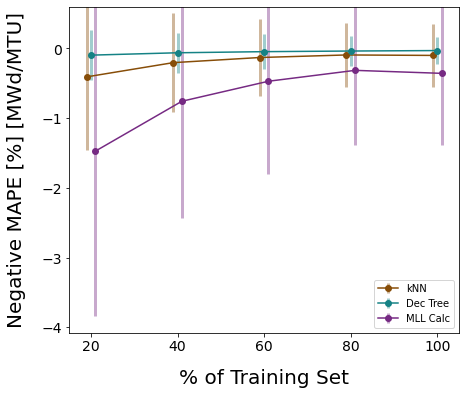
\includegraphics[width=\textwidth]{./chapters/exp1/learncurve_nuc29_MAPE_burn.png}
        \caption{Negative \gls{MAPE} of burnup regression with respect to 
                 to training set size.}
        \label{fig:learnsB}
    \end{subfigure}
    \vskip\baselineskip
    \begin{subfigure}[b]{0.49\textwidth}
        \centering
        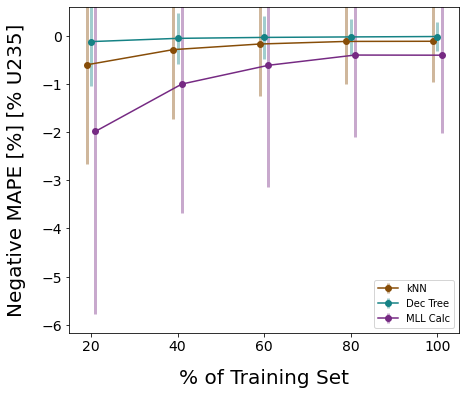
\includegraphics[width=\textwidth]{./chapters/exp1/learncurve_nuc29_MAPE_enri.png}
        \caption{Negative \gls{MAPE} of \gls{U235} enrichment regression with 
                 respect to training set size.}
        \label{fig:learnsC}
    \end{subfigure}
    \hfill
    \begin{subfigure}[b]{0.49\textwidth}
        \centering
        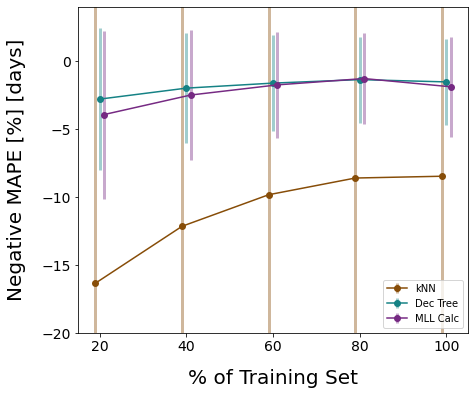
\includegraphics[width=\textwidth]{./chapters/exp1/learncurve_nuc29_MAPE_cool.png}
        \caption{Negative \gls{MAPE} of time since irradiation regression with 
                 respect to training set size.}
        \label{fig:learnsD}
    \end{subfigure}
    \caption{Learning curves for reactor type, burnup, enrichment, and time 
             since irradiation with respect to increasing fraction of the 
             training set.}
    \label{fig:learns}
\end{figure}

Although a key takeaway from Figure \ref{fig:randerr} is that the \gls{MLL}
calculations are the most robust to introduced error in the training set
features for all four prediction categories, there is another aspect of the
algorithm performance not shown in those plots: generalization. \Gls{MLL}
outperforms the scikit-learn methods in part because the training set is so
large. This is because it does not generalize to unseen data; it provides
predictions based on finding the closest training set entry to the test sample.
This is also true for the \textit{k}-nearest neighbor implementations where
$k=1$ (burnup and cooling time, as seen in Table \ref{tbl:exp1hypparam}).

One way to show that an algorithm is generalizing well in comparison to others
is to view the shape of its learning curve (introduced in Section
\ref{sec:complexity}): the prediction performance with respect to training set
size.  Learning curves were constructed for all four prediction categories,
demonstrated in Figure \ref{fig:learns}. As in Figure \ref{fig:randerr}, the
\textit{y}-axis is always oriented so that lower is poorer performance and
higher is better performance; also, the error bars reflect a 99\% confidence
interval for Figure \ref{fig:learnsA}, and one standard deviation of the
average percentage errors for Figures \ref{fig:learnsB}--\ref{fig:learnsD}.
These learning curves represent the 1\% random error case in Figure
\ref{fig:randerr}, so the \gls{MLL} learning curve will be below the
scikit-learn algorithms for the reactor type, burnup, and enrichment
predictions, and the \textit{k}-nearest neighbor learning curve will be below
the \gls{MLL} and decision tree curves for time since irradiation.  Thus, the
scores/errors in Figure \ref{fig:randerr} are the data points at the 100\%
training set level in Figure \ref{fig:learns}.  \todo[inline]{would it be
better to flip the x-axis so that performance degradation travels right as in
the random error plots?}

Figure \ref{fig:learnsA} shows that the balanced accuracy score of reactor type
classification for the \gls{MLL} calculations decreases more at lower training
set size than for the scikit-learn algorithms.  This pattern holds true for the
burnup \gls{MAPE} in Figure \ref{fig:learnsB} and the enrichment \gls{MAPE} in
Figure \ref{fig:learnsC}, although the standard deviation is large enough for
the \gls{MLL} values that the two sets of scikit-learn values are encompassed
by that range. Lastly, Figure \ref{fig:learnsD} has the error bars cropped out
for the \textit{k}-nearest neighbors curve in order to better see the \gls{MLL}
and decision tree curves. The latter two follow a nearly equivalent path, and
the decrease in performance for \textit{k}-nearest neighbors happens mostly in
parallel with them. As with the other regression cases, it is difficult to draw
a conclusion about the trend. While the 20\% and 40\% data points do seem to be
diverging faster, the error bars are too large to state anything definitive.

\noindent \textbf{Reactor Type Prior Knowledge}

There is similar work being done \todo{get tamu citation} to this that focuses
on these prediction categories but in a serial manner, i.e., first determining
the reactor type before moving forward with other predictions.
\todo[inline]{Finish intro here. Can't get the table to compile yet, so leaving
out for now}

\begin{figure}[!htb]
  \centering
  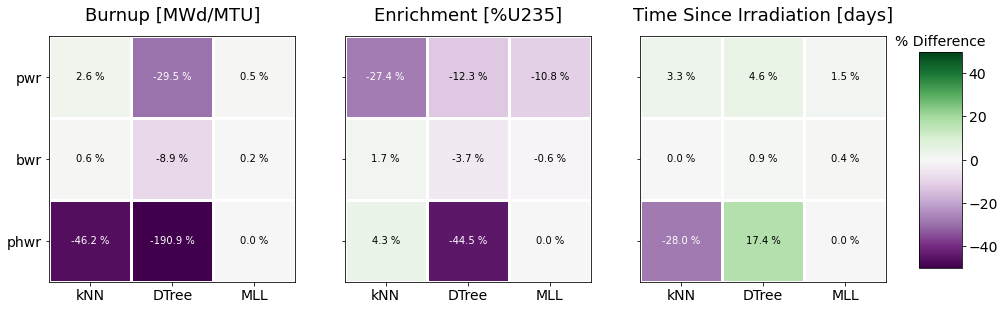
\includegraphics[width=1.1\textwidth]{./chapters/exp1/rxtr-type_known-unknown_diff.png}
  \caption{Heatmaps for the three regression cases showing the percent 
           difference in prediction error between a known reactor type 
           and unknown reactor type.}
  \label{fig:knownrxtr}
\end{figure}

%\begin{table}[!htb]
%  \centering
%  \begin{tabular}{@{}llllllll@{}} \toprule
%    \begin{tabular}[c]{@{}l@{}}Prediction\\ Parameter\end{tabular} 
%     & Reactor Type & kNN Known & kNN Unknown & DTree Known & DTree Unknown & MLL Known & MLL Unknown \\ \toprule
%    \multirow{3}{*}{\begin{tabular}[c]{@{}l@{}}Burnup\\ [MWd/MTU],\\ MAPE\end{tabular}}
%     & PWR & 0.08 & 0.08 & 0.03 & 0.04 & 0.24 & 0.25 \\
%     & BWR  & 0.11  & 0.10  & 0.03 & 0.03 & 0.40 & 0.40 \\
%     & PHWR & 0.13  & 0.19  & 0.01 & 0.03 & 0.29 & 0.29 \\ \midrule
%    \multirow{3}{*}{\begin{tabular}[c]{@{}l@{}}Enrichment\\ [\% U235], \\ MAPE\end{tabular}}
%     & PWR & 0.10 & 0.11 & 0.02 & 0.02 & 0.26 & 0.29 \\
%     & BWR  & 0.12  & 0.12  & 0.02 & 0.02 & 0.46 & 0.46 \\
%     & PHWR & 0.00  & 0.00  & 0.00 & 0.00 & 0.00 & 0.00 \\ \midrule
%    \multirow{3}{*}{\begin{tabular}[c]{@{}l@{}}Time Since \\ Irradiation\\ [days], \\ MAPE\end{tabular}}
%     & PWR & 6.47 & 6.13 & 1.50 & 1.43 & 1.55 & 1.46 \\
%     & BWR  & 9.18  & 9.15  & 1.56 & 1.53 & 2.07 & 2.05 \\
%     & PHWR & 13.78 & 18.62 & 4.51 & 3.71 & 2.30 & 2.30 \\ \bottomrule
%  \end{tabular}
%  \caption{Caption.}
%  \label{tbl:knownrxtr}
%\end{table}

The workflow was repeated for the three regression cases where they were
trained on reactor type-filtered training sets. A 1\% random error was applied
to these training sets, and the 1\% random error full training set was used as
comparison.  Figure \ref{fig:knownrxtr} is three heatmaps that show the percent
difference in prediction \gls{MAE} for each algorithm and reactor type between
the reactor type being known versus unknown prior to prediction. This is
reflected by a diverging color bar as well as a positive or negative percentage
in each square.  The positive percentages indicate the error decreased/improved
from the unknown reactor type case to the known reactor type case.  The
negative percentages indicate the error increased/worsened from the unknown to
the known case. 

For burnup prediction, most differences are within $\pm10\%$ except for three
scenarios.  The decision tree algorithm has improved burnup prediction for
\gls{PWR}s by almost 30\% and for \gls{PHWR}s by almost 200\% given a known
reactor type.  The \textit{k}-nearest neighbors algorithm has 46\% improved
burnup prediction for the \gls{PHWR}. For \gls{U235} enrichment, the \gls{PWR}
predictions all improve by over 10\%, including for the \gls{MLL} algorithm.
This is the only scenario where there is an appreciable difference in \gls{MLL}
performance. The decision tree enrichment prediction of \gls{PHWR}s also has a
sizeable improvement of 44\%.  The time since irradiation predictions for the
most part do not show improvement outside of $\pm10\%$. Of note is some
volatile behavior for the \gls{PHWR} case with the scikit-learn algorithms.
While \textit{k}-nearest neighbors improves by 28\%, the decision tree
predictions were worse by 17\%.

The improvements in the \gls{PHWR} predictions are not surprising since the
generalization of the scikit-learn algorithms could lead to the unique
\gls{PHWR} cases being ignored, since they are after all only 1.5\% of the
training set.  Another interesting result is that the \gls{BWR} predictions
experience no large changes, which makes sense given that they comprise 72\% of
the training set. Also, the \gls{MLL} predictions are approximately the same,
which is expected because this algorithm does not generalize, and the
prediction comes as a set of labels and is therefore already linked to the
reactor type.  The only confounding behavior is the performance decrease in the
\gls{PHWR} enrichment prediction by the decision tree method.  Overall, it is
important to be aware that the regression labels coming from a \gls{PHWR} will
be unlikely to be optimal results (except for those from \gls{MLL}
calculations).

\subsection{SFCOMPO Test Set}
\label{sec:sfcompo}

The testing described in Section \ref{sec:randerr} describes the process of
evaluating the methodology with test cases drawn from the training database.
It is also helpful to test the methodology against real assays of \gls{SNF}.
The \gls{SFCOMPO} database was created to allow access to these sorts of
measurements linked to the reactor operation parameters being predicted in this
work. The only parameter not part of the \gls{SFCOMPO} database is the time
since irradiation, so that is not predicted here. 

There are 505 test cases that are able to be compared against the training
database.  The number of each reactor type is as follows: 312 \gls{PWR}s, 165
\gls{BWR}s, and 28 \gls{PHWR}s. The space of enrichment and burnup values is
visualized in Figure \ref{fig:sfcoscatter}. These are sufficienty represented
in the training set design, as pictured in Figure \ref{fig:trainhist}.

\begin{figure}[!ht]
    \centering
    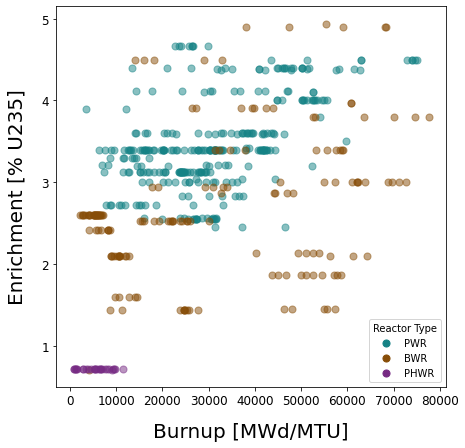
\includegraphics[width=0.7\textwidth]{./chapters/exp1/sfcompo_scatter_viz.png}
    \caption{Scatter plot showing the range of reactor operation parameters in 
             the \gls{SFCOMPO} testing set that are being predicted.}
    \label{fig:sfcoscatter}
    \todo[inline]{increase tick size, change order to bwr, pwr, phwr. Maybe show 
                  comparison against training E v B scatter plot}
\end{figure}



\begin{table}[!ht]
  \centering
  \begin{tabular}{@{}l|lll|lll@{}}
  \toprule
                   & \multicolumn{3}{l|}{Accuracy Scores} & \multicolumn{3}{l}{Balanced Accuracy Scores} \\ \toprule
  Null Handling    & kNN        & DTree      & MLL       & kNN           & DTree         & MLL           \\ \midrule
  Imputed Nulls    & 0.52       & 0.60       & 0.39      & 0.09          & 0.12          & 0.00          \\
  Zero-value Nulls & 0.45       & 0.42       & 0.72      & 0.21          & 0.30          & 0.63          \\ \bottomrule
  \end{tabular}
  \caption{sfcompo reactor accuracies.}
  \label{tbl:sfcorxtr}
\end{table}

\begin{figure}[!ht]
    \centering
    \begin{subfigure}[b]{0.49\textwidth}
        \centering
        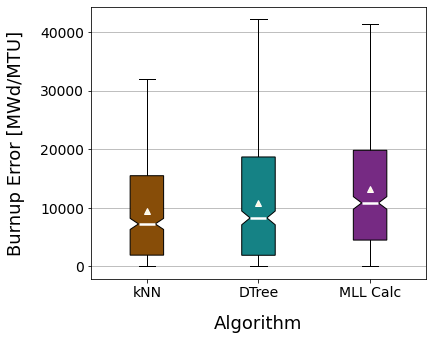
\includegraphics[width=\textwidth]{./chapters/exp1/sfcompo_boxplots_impnull_burn.png}
        \caption[]{Caption.}
        %\label{fig:}
    \end{subfigure}
    \hfill
    \begin{subfigure}[b]{0.49\textwidth}
        \centering
        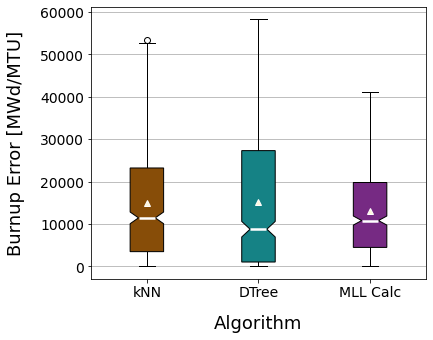
\includegraphics[width=\textwidth]{./chapters/exp1/sfcompo_boxplots_0null_burn.png}
        \caption[]{Caption.}
        %\label{fig:}
    \end{subfigure}
    \caption{sfcompo burnup boxplots.}
    \label{fig:sfcoburn}
\end{figure}

\begin{table}[!ht]
  \centering
  \begin{tabular}{@{}l|lll|lll@{}}
  \toprule
                   & \multicolumn{3}{l|}{Mean Errors [GWd/MTU]} & \multicolumn{3}{l}{Median Errors [GWd/MTU]} \\ \toprule
  Null Handling    & kNN           & DTree         & MLL           & kNN            & DTree          & MLL    \\ \midrule
  Imputed Nulls    & 9.43          & 10.89         & 13.17         & 7.26           & 8.28           & 10.84  \\
  Zero-value Nulls & 14.88         & 15.18         & 3.53          & 11.47          & 8.79           & 1.70   \\ \bottomrule
  \end{tabular}
  \caption{sfcompo burnup errors.}
  \label{tbl:sfcoburn}
\end{table}

\begin{figure}[!ht]
    \centering
    \begin{subfigure}[b]{0.49\textwidth}
        \centering
        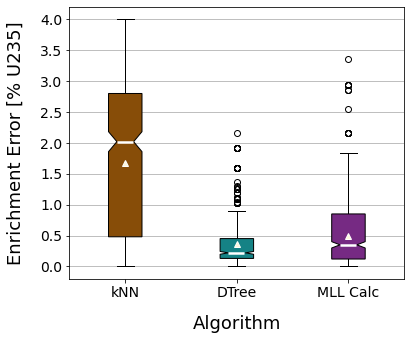
\includegraphics[width=\textwidth]{./chapters/exp1/sfcompo_boxplots_0null_enri.png}
        \caption[]{Caption.}
        %\label{fig:}
    \end{subfigure}
    \hfill
    \begin{subfigure}[b]{0.49\textwidth}
        \centering
        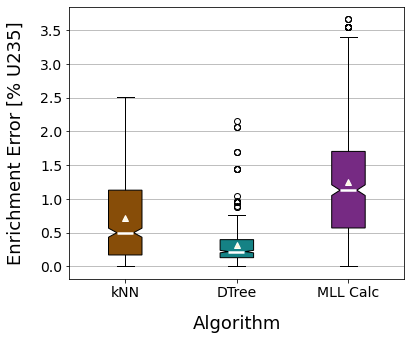
\includegraphics[width=\textwidth]{./chapters/exp1/sfcompo_boxplots_impnull_enri.png}
        \caption[]{Caption.}
        %\label{fig:}
    \end{subfigure}
    \caption{sfcompo enrichment boxplots.}
    \label{fig:sfcoenri}
\end{figure}

\begin{table}[!ht]
  \centering
  \begin{tabular}{@{}l|lll|lll@{}}
  \toprule
                   & \multicolumn{3}{l|}{Mean Errors [\% U235]} & \multicolumn{3}{l}{Median Errors [\% U235]} \\ \toprule
  Null Handling    & kNN           & DTree          & MLL          & kNN            & DTree          & MLL    \\ \midrule
  Imputed Nulls    & 0.72          & 0.31           & 1.25         & 0.50           & 0.22           & 1.13   \\
  Zero-value Nulls & 1.67          & 0.36           & 0.49         & 2.02           & 0.22           & 0.35   \\ \bottomrule
  \end{tabular}
  \caption{sfcompo enrichment errors.}
  \label{tbl:sfcoenri}
\end{table}

